
\documentclass{beamer} 


\mode<presentation>
{
  \usetheme{Berkeley}
  % or ...

  \setbeamercovered{transparent}
  % or whatever (possibly just delete it)
}

\usepackage{tikz}
\usepackage{graphicx}
\usepackage[english]{babel}
% or whatever

\usepackage[utf8]{inputenc}
% or whatever

\usepackage{times}
\usepackage[T1]{fontenc}
% Or whatever. Note that the encoding and the font should match. If T1
% does not look nice, try deleting the line with the fontenc.


\title[BITSS Update] % (optional, use only with long paper titles)
{BITSS Update}

\subtitle
{}

\author[Christensen] % (optional, use only with lots of authors)
{Garret~Christensen\inst{1}}
% - Give the names in the same order as the appear in the paper.
% - Use the \inst{?} command only if the authors have different
%   affiliation.

\institute[Universities of Somewhere and Elsewhere] % (optional, but mostly needed)
{
  \inst{1}%
  UC Berkeley:\\
  Berkeley Initiative for Transparency in the Social Sciences\\
  Berkeley Institute for Data Science\\
  }
% - Use the \inst command only if there are several affiliations.
% - Keep it simple, no one is interested in your street address.

\date[BITSS2014] % (optional, should be abbreviation of conference name)
{CEGA Staff, October 2016\\
Slides available online at \url{http://www.github.com/BITSS/projectupdate}}
% - Either use conference name or its abbreviation.
% - Not really informative to the audience, more for people (including
%   yourself) who are reading the slides online

\subject{Research Transparency}
% This is only inserted into the PDF information catalog. Can be left
% out. 

\pgfdeclareimage[height=2cm]{university-logo}{../Images/BITSSlogo.png}
\logo{\pgfuseimage{university-logo}}

% If you have a file called "university-logo-filename.xxx", where xxx
% is a graphic format that can be processed by latex or pdflatex,
% resp., then you can add a logo as follows:

% \pgfdeclareimage[height=0.5cm]{university-logo}{university-logo-filename}
% \logo{\pgfuseimage{university-logo}}



% Delete this, if you do not want the table of contents to pop up at
% the beginning of each subsection:
%\AtBeginSubsection[]
%{
%  \begin{frame}<beamer>{Outline}
%    \tableofcontents[currentsection,currentsubsection]
%  \end{frame}
%}


% If you wish to uncover everything in a step-wise fashion, uncomment
% the following command: 

\beamerdefaultoverlayspecification{<+->}


\begin{document}

\begin{frame}
  \titlepage
\end{frame}




% Structuring a talk is a difficult task and the following structure
% may not be suitable. Here are some rules that apply for this
% solution: 

% - Exactly two or three sections (other than the summary).
% - At *most* three subsections per section.
% - Talk about 30s to 2min per frame. So there should be between about
%   15 and 30 frames, all told.

% - A conference audience is likely to know very little of what you
%   are going to talk about. So *simplify*!
% - In a 20min talk, getting the main ideas across is hard
%   enough. Leave out details, even if it means being less precise than
%   you think necessary.
% - If you omit details that are vital to the proof/implementation,
%   just say so once. Everybody will be happy with that.
%%%%%%%%%%%%%%%%%%%%%%%%%%%%%%%%%%%%%%%%%%%%%%%%%%%%%%%%%%%%%%%%%%%%%%%
%%%%%%%%%%%%%%%%%%%%%%%%%%%%%%%%%%%%%%%%%%%%%%%%%%%%%%%%%%%%%%%%%%%%%
\begin{frame}{Outline}
  \tableofcontents
  % You might wish to add the option [pausesections]
\end{frame}
\section {Introduction}
{ % all template changes are local to this group.
    \setbeamertemplate{navigation symbols}{}
    \begin{frame}[plain]
        \begin{tikzpicture}[remember picture,overlay]
            \node[at=(current page.center)] {
                \href{https://www.bitss.org/}{
\includegraphics[width=\paperwidth]{../Images/BITSSlogo.png}}
            };
        \end{tikzpicture}
     \end{frame}
}

%%%%%%%%%%%%%%%%%%%%%%%%%%%%%%%%%%%%%%%%%%%%%%%%%%%%%%%%%%%%%%%%%%%%%%%%%%%%%%%%%%%

%%%%%%%%%%%%%%%%%%%%%%%%%%%%%%%%%%%%%%%%%%%%%%%%%%%%%%%%%%%%%%%%%%

%%%%%%%%%%%%%%%%%%%%%%%%%%%%%%%%%%%%%%%%%%%%%%%%%%%%%%%%%%%%%%%%%%%%%


\begin{frame}{Registration}
 Newer to social sciences, but:
   \begin{itemize}[<.->]
   \item
   	AEA registry, currently only for RCTs. \url{http://socialscienceregistry.org}
   \item
    EGAP registry \url{http://egap.org/design-registration}
   \item 
    3ie registry, for developing country evaluations. \url{http://ridie.3ieimpact.org}
   \item
   	Open Science Framework\\ \url{http://osf.io}
   	\begin{itemize}
   	\item
   	Open format
   	\item
   	Will soon sync with above
   	\end{itemize}
   	\item Simple: \url{http://aspredicted.org}
   \end{itemize}
 
\end{frame}

 { % all template changes are local to this group.
    \setbeamertemplate{navigation symbols}{}
    \begin{frame}[plain, label=AEAreg]
         \begin{tikzpicture}[remember picture,overlay]
            \node[at=(current page.center)] {
                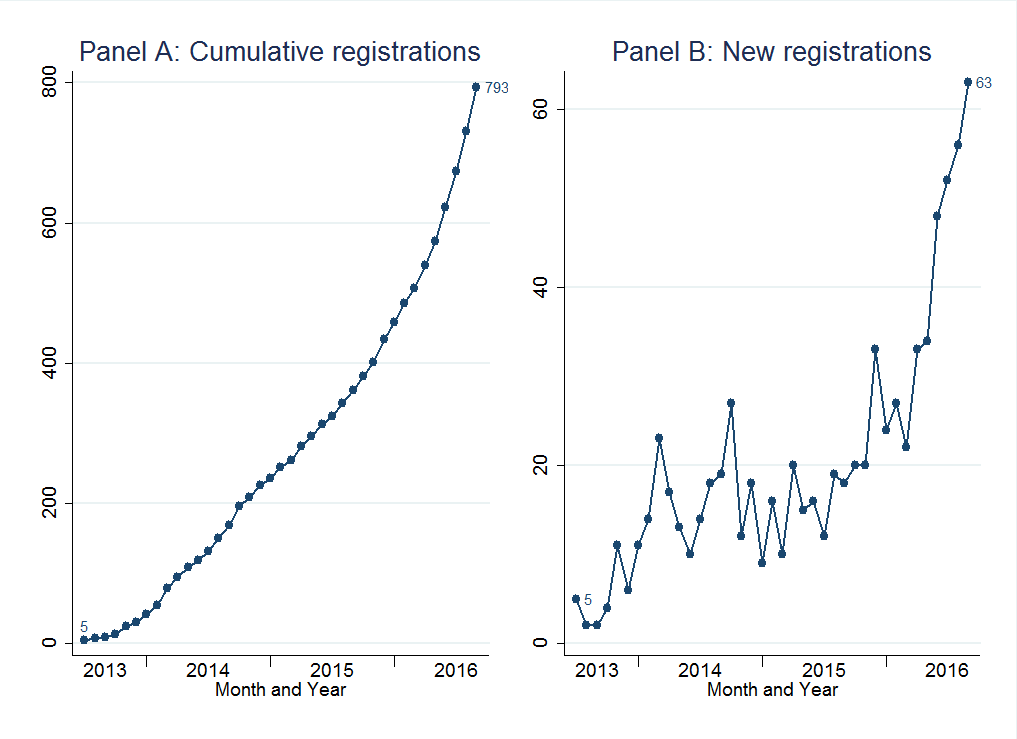
\includegraphics[height=\paperheight]{../Images/AEARegistrations.PNG}
            };
        \end{tikzpicture}
     \end{frame}
}

\begin{frame}{Design-Based Publication}
AKA Registered Reports, moves peer review before data gathering, results, and analysis.

\begin{enumerate}[<.->]
\item Design a project
\item Submit
\item Reviewed based on importance of question and quality of design
\item Get in-principle acceptance
\item Follow through, and nulls get published
\end{enumerate}
\href{https://osf.io/8mpji/wiki/home/}{20 Journals, 5 more with Special Issues \beamergotobutton{Link}}
\end{frame}

{ % all template changes are local to this group.
    \setbeamertemplate{navigation symbols}{}
    \begin{frame}[plain, label=AEAreg]
         \begin{tikzpicture}[remember picture,overlay]
            \node[at=(current page.center)] {
                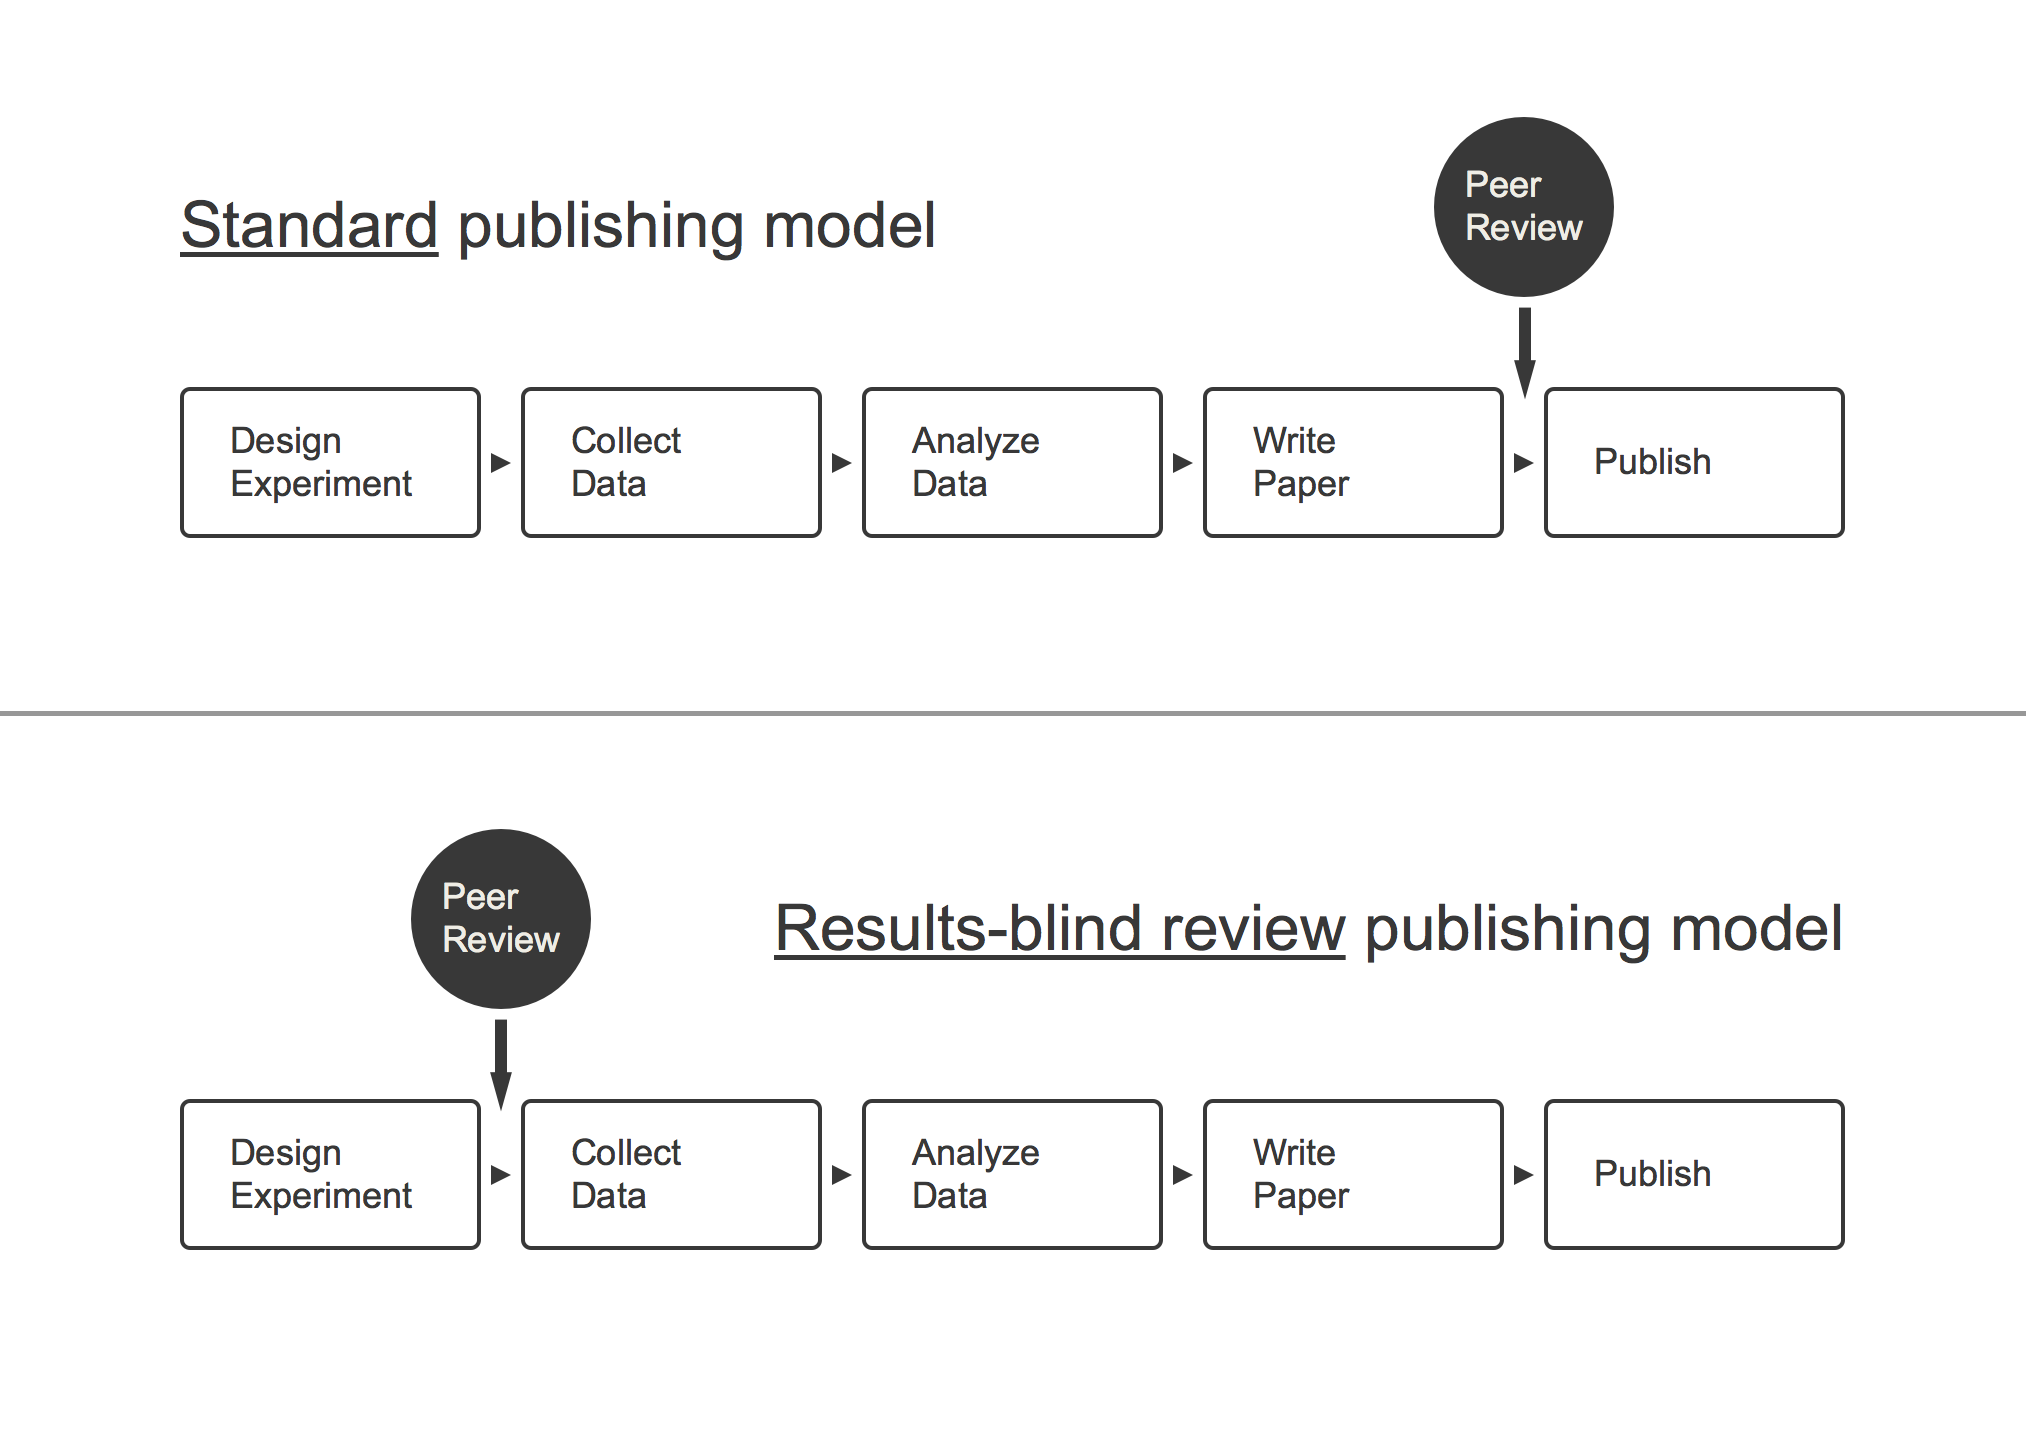
\includegraphics[height=\paperheight]{../Images/results_blind_review.png}
            };
        \end{tikzpicture}
     \end{frame}
}

\begin{frame}{P-Hacking is fun!}
\begin{itemize}
\item
``Science isn't Broken'' ---538 journalism piece with interactive demo \href{http://fivethirtyeight.com/features/science-isnt-broken}{\beamerbutton{Link}}
\item 
Train your p-hacking skills R/Shiny App. \href{http://www.nicebread.de/introducing-p-hacker/}{\beamerbutton{Link}}
\item
An Exact Fishy Test \href{https://macartan.shinyapps.io/fish/}{\beamerbutton{Link}}
\end{itemize}
\end{frame}


{ % all template changes are local to this group.
    \setbeamertemplate{navigation symbols}{}
    \begin{frame}[plain]
         \begin{tikzpicture}[remember picture,overlay]
            \node[at=(current page.center)] {
                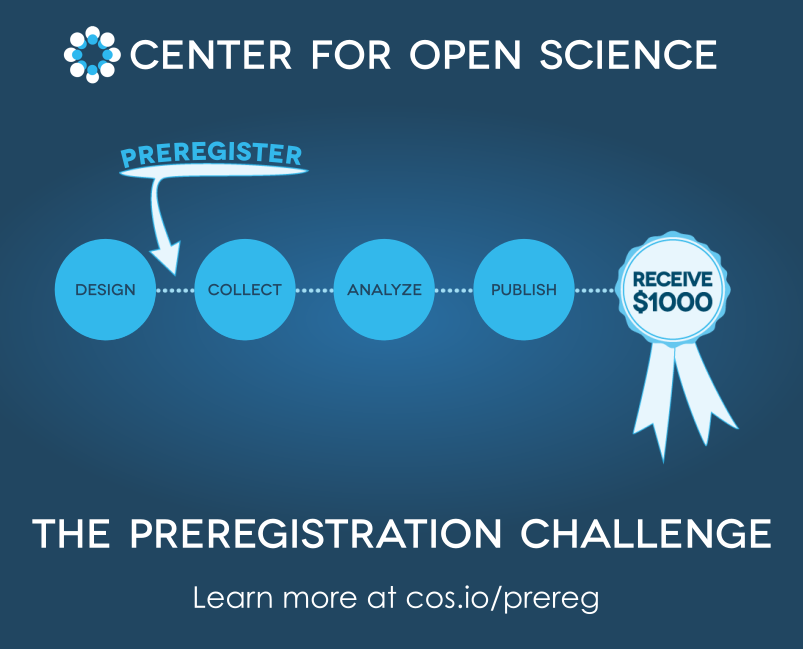
\includegraphics[width=\paperwidth]{../Images/preregchallenge.png}
            };
        \end{tikzpicture}
     \end{frame}
}
%%%%%%%%%%%%%%%%%%%%%%%%%%%%%%%%%%%%%%%%%%%%%%%%%%%%

%%%%%%%%%%%%%%%%%%%%%%%%%%%%%%%%%%%%%%%%%%%%%%%%%%%%%%%%%%%%%%%%%%%%

 { % all template changes are local to this group.
    \setbeamertemplate{navigation symbols}{}
    \begin{frame}[plain, label=AEAreg]
         \begin{tikzpicture}[remember picture,overlay]
            \node[at=(current page.center)] {
                
\includegraphics[width=\paperwidth]{../Images/TOPGuidelines.PNG}
            };
        \end{tikzpicture}
     \end{frame}
}

\subsection*{Version Control}
\begin{frame}{Version Control}
\begin{itemize}[<.->]
\item
Using version control (AKA revision control) can help to make your work more reproducible.

\item
What is version control?

\begin{quote}
Version control is a system that records changes to a file or set of files over time so that you can recall specific versions later. For the examples in this book you will use software source code as the files being version controlled, though in reality you can do this with nearly any type of file on a computer.
\end{quote}
--Git, \href{https://git-scm.com/book/en/v2/Getting-Started-About-Version-Control}{About Version Control}
%\item Distributed Version Control Systems (DCVS) let multiple users control the same files in this manner.
\end{itemize}
\end{frame}

 { % all template changes are local to this group.
    \setbeamertemplate{navigation symbols}{}
    \begin{frame}[plain, label=AEAreg]
         \begin{tikzpicture}[remember picture,overlay]
            \node[at=(current page.center)] {
                
\includegraphics[height=\paperheight]{../Images/github-logo-transparent.JPG}
            };
        \end{tikzpicture}
     \end{frame}

 % all template changes are local to this group.
    \setbeamertemplate{navigation symbols}{}
    \begin{frame}[plain]
         \begin{tikzpicture}[remember picture,overlay]
            \node[at=(current page.center)] {
                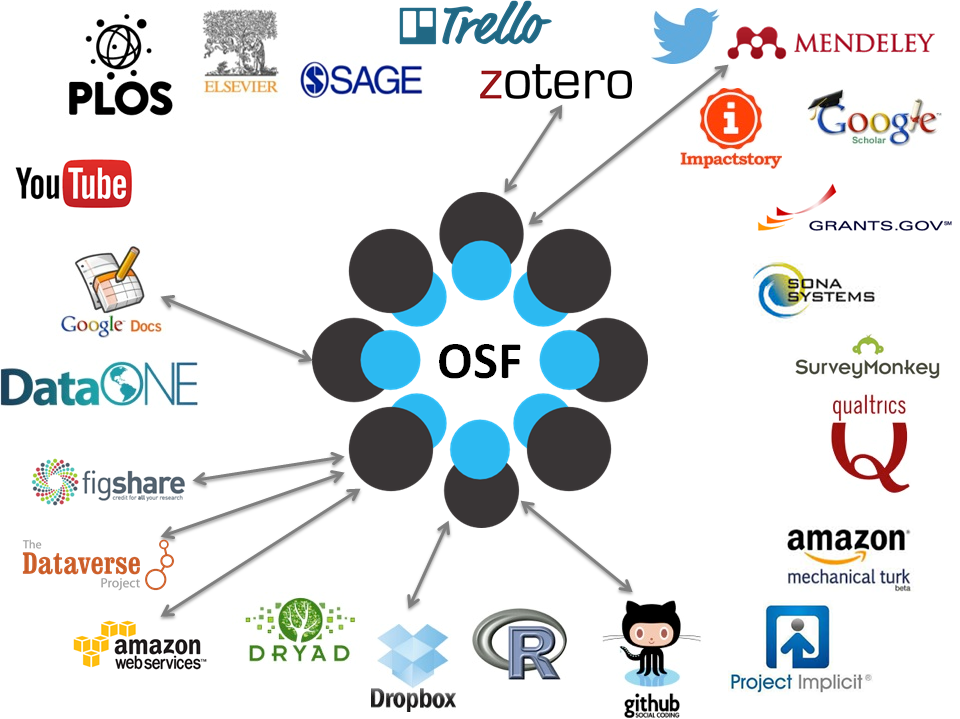
\includegraphics[width=\paperwidth]{../Images/OSFnow.PNG}
            };
        \end{tikzpicture}
     \end{frame}

% all template changes are local to this group.
    \setbeamertemplate{navigation symbols}{}
    \begin{frame}[plain]
         \begin{tikzpicture}[remember picture,overlay]
            \node[at=(current page.center)] {
                
\includegraphics[width=\paperwidth]{../Images/OSFsoon.PNG}
            };
        \end{tikzpicture}
     \end{frame}

}


\begin{frame}{Dynamic Documents}
Write your code and your paper in the same file so you won't lose information or make copy and paste mistakes.

Possible in R and Stata.
\begin{itemize}[<.->]
\item Include tables by linking to a file, instead of a static image.
\item Include number by linking to a value calculated by an analysis file, instead of a static number typed manually.
\item Automatically update tables and numbers.
\item Produce entire paper with one or two clicks.
\end{itemize} 
\end{frame}


 { % all template changes are local to this group.
    \setbeamertemplate{navigation symbols}{}
    \begin{frame}[plain, label=AEAreg]
         \begin{tikzpicture}[remember picture,overlay]
            \node[at=(current page.center)] {
                
\includegraphics[height=\paperheight]{../Images/jupyter.png}
            };
        \end{tikzpicture}
     \end{frame}
}
 { % all template changes are local to this group.
    \setbeamertemplate{navigation symbols}{}
    \begin{frame}[plain, label=AEAreg]
         \begin{tikzpicture}[remember picture,overlay]
            \node[at=(current page.center)] {
                
\includegraphics[width=\paperwidth]{../Images/RStudio-Logo-Blue-Gradient.png}
            };
        \end{tikzpicture}
     \end{frame}
}

\section{Conclusion}
\begin{frame}{Conclusion}
OK, I'm convinced. How do I implement this in my own research?

\begin{itemize}[<.->]
\item Read the manual I wrote.\href{https://github.com/garretchristensen/BestPracticesManual}{\beamergotobutton{Link}}
\item Subscribe to the BITSS blog \& E-mail list \href{https://bitss.org/blog}{\beamergotobutton{Link}}
\item Apply for our NIH Summer Institute. \href{http://www.bitss.org/events/summer-institute/}{\beamergotobutton{Link}}
\item Apply for our SSMART Grants (extra funding for developing country researchers). \href{http://www.bitss.org/ssmart-grants/}{\beamergotobutton{Link}}
\item Apply for our Leamer-Rosenthal Prizes. \href{http://www.bitss.org/lr-prizes/}{\beamergotobutton{Link}}
\item Free stats consulting from COS. \href{https://cos.io/stats_consulting/}{\beamergotobutton{Link}}
\end{itemize}
\end{frame}

\begin{frame}{Summer Institute}
Three days of training in June at UC Berkeley, or two days of training in July at the University of Michigan.
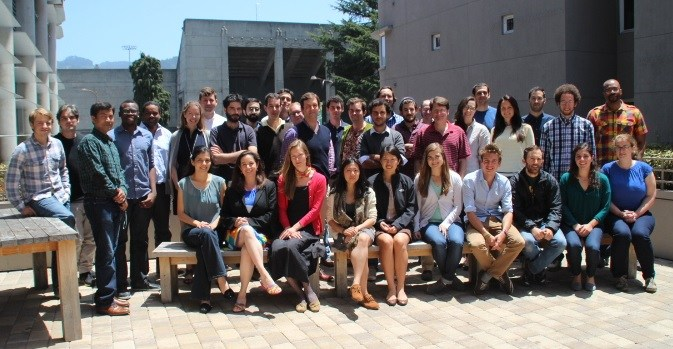
\includegraphics[width=4in]{../Images/bitss-2014-cohort2.jpg}
\end{frame}

\begin{frame}{SSMART Grant}
Up to \$30,000 grant for a research project on:
\begin{itemize}[<.->]
\item Develop new methodology
\item New tools and approaches for meta-analysis
\item Research on researchers and adoption of new norms
\end{itemize}
Extra funding source for researchers from developing countries.

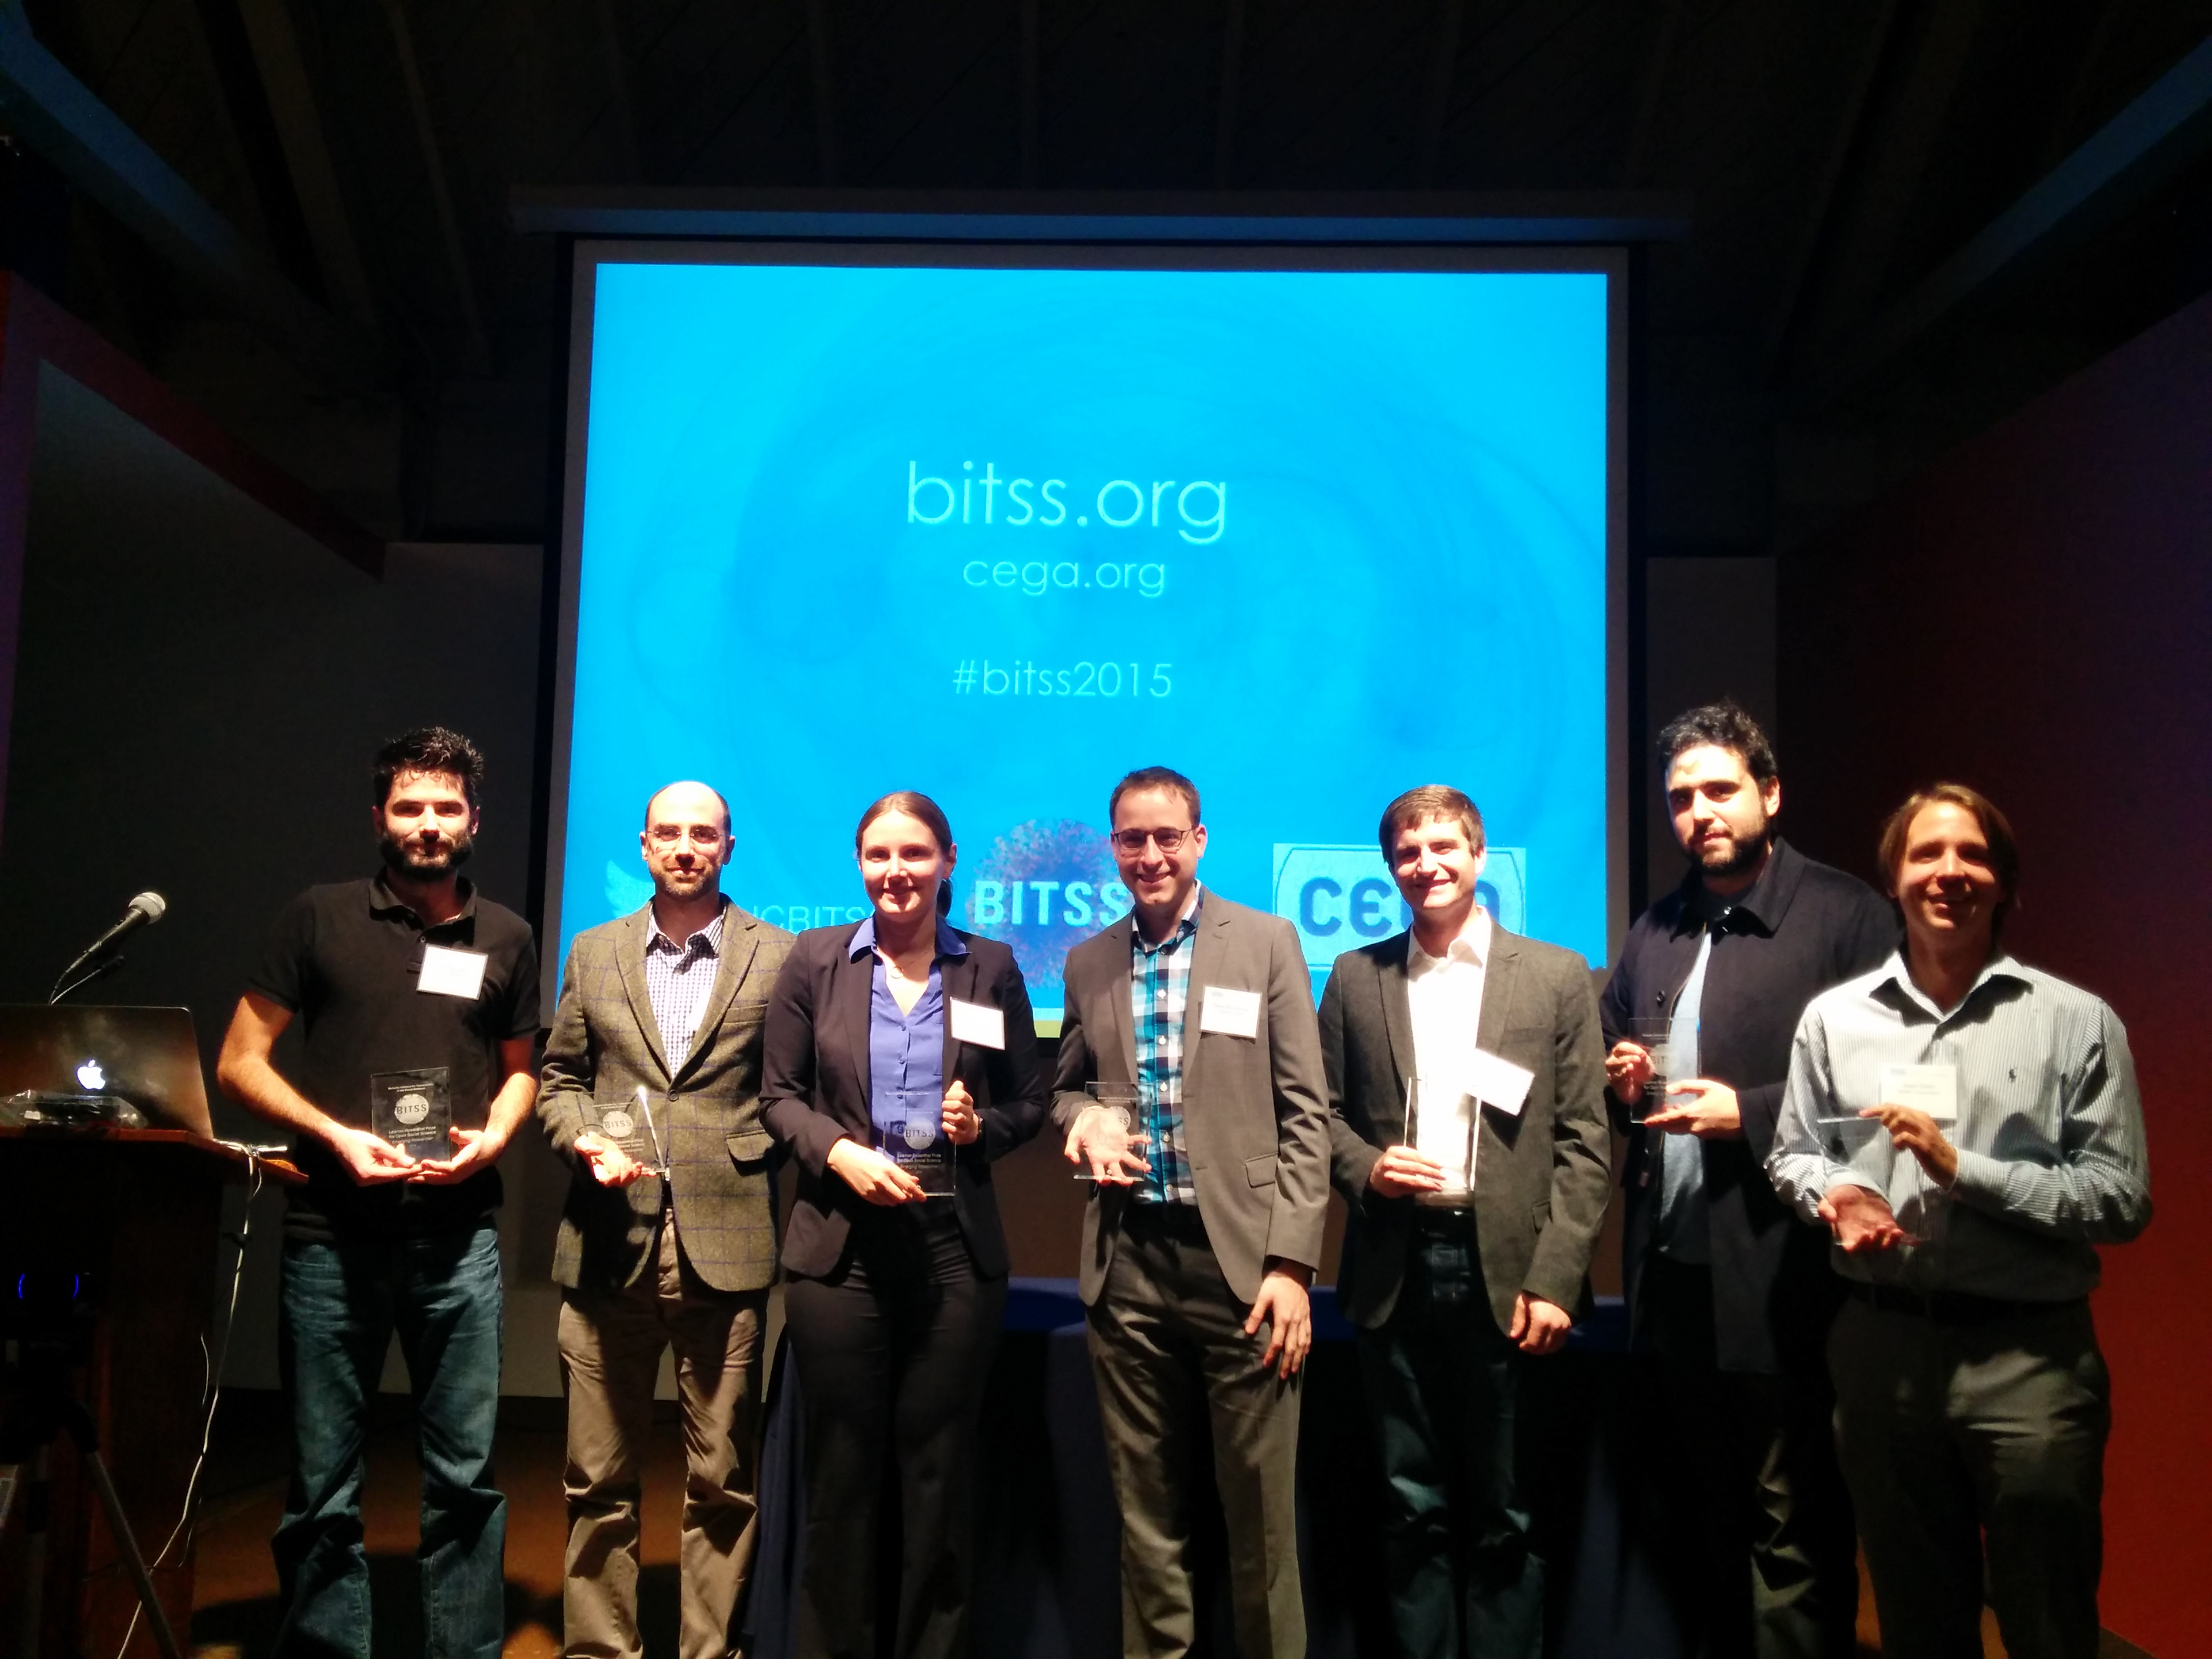
\includegraphics[width=2.5in]{../Images/LRwinners.jpg}
\end{frame}

\begin{frame}{Leamer-Rosenthal Prizes}
Up to \$10,000 prize for completed transparent research in the social sciences,
especially:
\begin{itemize}[<.->]
\item Economics
\item Political Science
\item Psychology
\end{itemize}
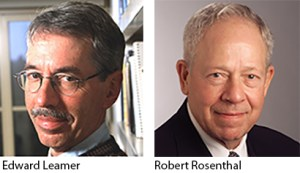
\includegraphics[width=2.5in]{../Images/leamer1-zoomed33.jpg}
\end{frame}


\begin{frame}
\begin{center}
Questions?
\vspace{1in}


\Huge{Thank you!}
\end{center}
\end{frame}

\end{document}

